% Options for packages loaded elsewhere
\PassOptionsToPackage{unicode}{hyperref}
\PassOptionsToPackage{hyphens}{url}
%
\documentclass[
]{article}
\usepackage{amsmath,amssymb}
\usepackage{lmodern}
\usepackage{ifxetex,ifluatex}
\ifnum 0\ifxetex 1\fi\ifluatex 1\fi=0 % if pdftex
  \usepackage[T1]{fontenc}
  \usepackage[utf8]{inputenc}
  \usepackage{textcomp} % provide euro and other symbols
\else % if luatex or xetex
  \usepackage{unicode-math}
  \defaultfontfeatures{Scale=MatchLowercase}
  \defaultfontfeatures[\rmfamily]{Ligatures=TeX,Scale=1}
\fi
% Use upquote if available, for straight quotes in verbatim environments
\IfFileExists{upquote.sty}{\usepackage{upquote}}{}
\IfFileExists{microtype.sty}{% use microtype if available
  \usepackage[]{microtype}
  \UseMicrotypeSet[protrusion]{basicmath} % disable protrusion for tt fonts
}{}
\makeatletter
\@ifundefined{KOMAClassName}{% if non-KOMA class
  \IfFileExists{parskip.sty}{%
    \usepackage{parskip}
  }{% else
    \setlength{\parindent}{0pt}
    \setlength{\parskip}{6pt plus 2pt minus 1pt}}
}{% if KOMA class
  \KOMAoptions{parskip=half}}
\makeatother
\usepackage{xcolor}
\IfFileExists{xurl.sty}{\usepackage{xurl}}{} % add URL line breaks if available
\IfFileExists{bookmark.sty}{\usepackage{bookmark}}{\usepackage{hyperref}}
\hypersetup{
  pdftitle={Distribuciones notables discretas},
  pdfauthor={Christian Limbert Paredes Aguilera},
  hidelinks,
  pdfcreator={LaTeX via pandoc}}
\urlstyle{same} % disable monospaced font for URLs
\usepackage[margin=1in]{geometry}
\usepackage{color}
\usepackage{fancyvrb}
\newcommand{\VerbBar}{|}
\newcommand{\VERB}{\Verb[commandchars=\\\{\}]}
\DefineVerbatimEnvironment{Highlighting}{Verbatim}{commandchars=\\\{\}}
% Add ',fontsize=\small' for more characters per line
\usepackage{framed}
\definecolor{shadecolor}{RGB}{248,248,248}
\newenvironment{Shaded}{\begin{snugshade}}{\end{snugshade}}
\newcommand{\AlertTok}[1]{\textcolor[rgb]{0.94,0.16,0.16}{#1}}
\newcommand{\AnnotationTok}[1]{\textcolor[rgb]{0.56,0.35,0.01}{\textbf{\textit{#1}}}}
\newcommand{\AttributeTok}[1]{\textcolor[rgb]{0.77,0.63,0.00}{#1}}
\newcommand{\BaseNTok}[1]{\textcolor[rgb]{0.00,0.00,0.81}{#1}}
\newcommand{\BuiltInTok}[1]{#1}
\newcommand{\CharTok}[1]{\textcolor[rgb]{0.31,0.60,0.02}{#1}}
\newcommand{\CommentTok}[1]{\textcolor[rgb]{0.56,0.35,0.01}{\textit{#1}}}
\newcommand{\CommentVarTok}[1]{\textcolor[rgb]{0.56,0.35,0.01}{\textbf{\textit{#1}}}}
\newcommand{\ConstantTok}[1]{\textcolor[rgb]{0.00,0.00,0.00}{#1}}
\newcommand{\ControlFlowTok}[1]{\textcolor[rgb]{0.13,0.29,0.53}{\textbf{#1}}}
\newcommand{\DataTypeTok}[1]{\textcolor[rgb]{0.13,0.29,0.53}{#1}}
\newcommand{\DecValTok}[1]{\textcolor[rgb]{0.00,0.00,0.81}{#1}}
\newcommand{\DocumentationTok}[1]{\textcolor[rgb]{0.56,0.35,0.01}{\textbf{\textit{#1}}}}
\newcommand{\ErrorTok}[1]{\textcolor[rgb]{0.64,0.00,0.00}{\textbf{#1}}}
\newcommand{\ExtensionTok}[1]{#1}
\newcommand{\FloatTok}[1]{\textcolor[rgb]{0.00,0.00,0.81}{#1}}
\newcommand{\FunctionTok}[1]{\textcolor[rgb]{0.00,0.00,0.00}{#1}}
\newcommand{\ImportTok}[1]{#1}
\newcommand{\InformationTok}[1]{\textcolor[rgb]{0.56,0.35,0.01}{\textbf{\textit{#1}}}}
\newcommand{\KeywordTok}[1]{\textcolor[rgb]{0.13,0.29,0.53}{\textbf{#1}}}
\newcommand{\NormalTok}[1]{#1}
\newcommand{\OperatorTok}[1]{\textcolor[rgb]{0.81,0.36,0.00}{\textbf{#1}}}
\newcommand{\OtherTok}[1]{\textcolor[rgb]{0.56,0.35,0.01}{#1}}
\newcommand{\PreprocessorTok}[1]{\textcolor[rgb]{0.56,0.35,0.01}{\textit{#1}}}
\newcommand{\RegionMarkerTok}[1]{#1}
\newcommand{\SpecialCharTok}[1]{\textcolor[rgb]{0.00,0.00,0.00}{#1}}
\newcommand{\SpecialStringTok}[1]{\textcolor[rgb]{0.31,0.60,0.02}{#1}}
\newcommand{\StringTok}[1]{\textcolor[rgb]{0.31,0.60,0.02}{#1}}
\newcommand{\VariableTok}[1]{\textcolor[rgb]{0.00,0.00,0.00}{#1}}
\newcommand{\VerbatimStringTok}[1]{\textcolor[rgb]{0.31,0.60,0.02}{#1}}
\newcommand{\WarningTok}[1]{\textcolor[rgb]{0.56,0.35,0.01}{\textbf{\textit{#1}}}}
\usepackage{graphicx}
\makeatletter
\def\maxwidth{\ifdim\Gin@nat@width>\linewidth\linewidth\else\Gin@nat@width\fi}
\def\maxheight{\ifdim\Gin@nat@height>\textheight\textheight\else\Gin@nat@height\fi}
\makeatother
% Scale images if necessary, so that they will not overflow the page
% margins by default, and it is still possible to overwrite the defaults
% using explicit options in \includegraphics[width, height, ...]{}
\setkeys{Gin}{width=\maxwidth,height=\maxheight,keepaspectratio}
% Set default figure placement to htbp
\makeatletter
\def\fps@figure{htbp}
\makeatother
\setlength{\emergencystretch}{3em} % prevent overfull lines
\providecommand{\tightlist}{%
  \setlength{\itemsep}{0pt}\setlength{\parskip}{0pt}}
\setcounter{secnumdepth}{-\maxdimen} % remove section numbering
\ifluatex
  \usepackage{selnolig}  % disable illegal ligatures
\fi

\title{Distribuciones notables discretas}
\author{Christian Limbert Paredes Aguilera}
\date{23/12/2021}

\begin{document}
\maketitle

\#library source(``funciones.R'')

\hypertarget{distribuciuxf3n-bernoulli}{%
\subsection{Distribución Bernoulli}\label{distribuciuxf3n-bernoulli}}

\begin{itemize}
  \item Consideremos un experemento con dos resultados posibles éxito (E) y fracaso (F). El espacio de sucesos será $\Omega = \lbrace E,F\rbrace$
  \item Supongamos que la probabilidad de éxito es $P(E) = p,$ y naturalmente $P(E)=1-p=q$ con $0<p<1$.
  \item Consideremos la aplicación $$X:\Omega = \lbrace E,F\rbrace \longrightarrow \mathbb{R}$$
  definida por $$E(X)=1,\quad X(F)=0$$
\end{itemize}

Su función de probabilidad es \[P_X(x) = \left\{\begin{array}{rcl}
  1-p=q&si&x=0\\
  p&si&x=1\\
  0&si&\mbox{en cualquier otro caso}\\
\end{array}\right.\]

Su función de distribución es

\[P_X(x) = \left\{\begin{array}{rcl}
  0&si&x<0\\
  1-p=q&si&0\leq x<1\\
  1&si&1\leq x\\
\end{array}\right.\]

\begin{itemize}
  \item Lo denotaremos por $$X\equiv Ber(p) \quad o\quad X\equiv B(1,p)$$
  \item a este tipo de experimentos (éxito/fracaso) se les denomina experimentos Bernoulli.
\end{itemize}

\hypertarget{esperanza-de-una-v.a.-x-berp}{%
\subsubsection{Esperanza de una v.a. X
Ber(p)}\label{esperanza-de-una-v.a.-x-berp}}

Su valor esperado es
\[E(X) = \sum_{x=0}^1 x\cdot P(X=x) = 0\cdot(1-p)+1\cdot p = p\]

Calculemos también \(E(X^2)\)
\[E(X^2) = \sum_{x=o}^1 x\cdot P(X=x) = 0^2 \cdot (1-p) + 1^2\cdot p = p\]

\hypertarget{varianza-de-una-v.a.-x-berp}{%
\subsubsection{Varianza de una v.a. X
Ber(p)}\label{varianza-de-una-v.a.-x-berp}}

Su varianza es
\[Var(X) = E(X^2) - E^2(X) = p-p^2 = p\cdot (1-p) = p\cdot q\]

Su desviación típica es \[\sqrt{Var(X)}=\sqrt{p\cdot (1-p)}\]

\begin{Shaded}
\begin{Highlighting}[]
\CommentTok{\#función de probabilidad}
\FunctionTok{dbinom}\NormalTok{(}\DecValTok{0}\NormalTok{, }\AttributeTok{size =} \DecValTok{1}\NormalTok{, }\AttributeTok{prob =} \FloatTok{0.25}\NormalTok{)}
\end{Highlighting}
\end{Shaded}

\begin{verbatim}
## [1] 0.75
\end{verbatim}

\begin{Shaded}
\begin{Highlighting}[]
\CommentTok{\#función de probabilidad}
\FunctionTok{dbinom}\NormalTok{(}\DecValTok{1}\NormalTok{, }\AttributeTok{size =} \DecValTok{1}\NormalTok{, }\AttributeTok{prob =} \FloatTok{0.25}\NormalTok{)}
\end{Highlighting}
\end{Shaded}

\begin{verbatim}
## [1] 0.25
\end{verbatim}

\begin{Shaded}
\begin{Highlighting}[]
\CommentTok{\# muestra aleatoria simple de probabilidad Bernoulli}
\FunctionTok{rbinom}\NormalTok{(}\AttributeTok{n =} \DecValTok{20}\NormalTok{, }\AttributeTok{size =} \DecValTok{1}\NormalTok{, }\AttributeTok{prob =} \FloatTok{0.25}\NormalTok{)}
\end{Highlighting}
\end{Shaded}

\begin{verbatim}
##  [1] 1 0 0 0 0 0 0 1 0 0 0 0 0 0 0 0 1 1 0 1
\end{verbatim}

\begin{Shaded}
\begin{Highlighting}[]
\CommentTok{\# gráfico de la función de probabilidad y la de distribución de una Ber(p=0.25)}
\NormalTok{\{}\FunctionTok{par}\NormalTok{(}\AttributeTok{mfrow=}\FunctionTok{c}\NormalTok{(}\DecValTok{1}\NormalTok{,}\DecValTok{2}\NormalTok{))}
\FunctionTok{plot}\NormalTok{(}\AttributeTok{x=}\FunctionTok{c}\NormalTok{(}\DecValTok{0}\NormalTok{,}\DecValTok{1}\NormalTok{),}\AttributeTok{y=}\FunctionTok{dbinom}\NormalTok{(}\FunctionTok{c}\NormalTok{(}\DecValTok{0}\NormalTok{,}\DecValTok{1}\NormalTok{),}\AttributeTok{size=}\DecValTok{1}\NormalTok{,}\AttributeTok{prob=}\FloatTok{0.25}\NormalTok{),}
     \AttributeTok{ylim=}\FunctionTok{c}\NormalTok{(}\DecValTok{0}\NormalTok{,}\DecValTok{1}\NormalTok{),}\AttributeTok{xlim=}\FunctionTok{c}\NormalTok{(}\SpecialCharTok{{-}}\DecValTok{1}\NormalTok{,}\DecValTok{2}\NormalTok{),}\AttributeTok{xlab=}\StringTok{"x"}\NormalTok{,}
     \AttributeTok{main=}\StringTok{"Función de probabilidad}\SpecialCharTok{\textbackslash{}n}\StringTok{ Ber(p=0.25)"}\NormalTok{)}
\FunctionTok{lines}\NormalTok{(}\AttributeTok{x=}\FunctionTok{c}\NormalTok{(}\DecValTok{0}\NormalTok{,}\DecValTok{0}\NormalTok{,}\DecValTok{1}\NormalTok{,}\DecValTok{1}\NormalTok{),}\AttributeTok{y=}\FunctionTok{c}\NormalTok{(}\DecValTok{0}\NormalTok{,}\FloatTok{0.75}\NormalTok{,}\DecValTok{0}\NormalTok{,}\FloatTok{0.25}\NormalTok{), }\AttributeTok{type =} \StringTok{"h"}\NormalTok{, }\AttributeTok{lty =} \DecValTok{2}\NormalTok{,}\AttributeTok{col=}\StringTok{"blue"}\NormalTok{)}
\FunctionTok{curve}\NormalTok{(}\FunctionTok{pbinom}\NormalTok{(x,}\AttributeTok{size=}\DecValTok{1}\NormalTok{,}\AttributeTok{prob=}\FloatTok{0.25}\NormalTok{),}
      \AttributeTok{xlim=}\FunctionTok{c}\NormalTok{(}\SpecialCharTok{{-}}\DecValTok{1}\NormalTok{,}\DecValTok{2}\NormalTok{),}\AttributeTok{col=}\StringTok{"blue"}\NormalTok{,}
      \AttributeTok{main=}\StringTok{"Función de distribución}\SpecialCharTok{\textbackslash{}n}\StringTok{ Ber(p=0.25)"}\NormalTok{)}
\FunctionTok{par}\NormalTok{(}\AttributeTok{mfrow=}\FunctionTok{c}\NormalTok{(}\DecValTok{1}\NormalTok{,}\DecValTok{1}\NormalTok{))\}}
\end{Highlighting}
\end{Shaded}

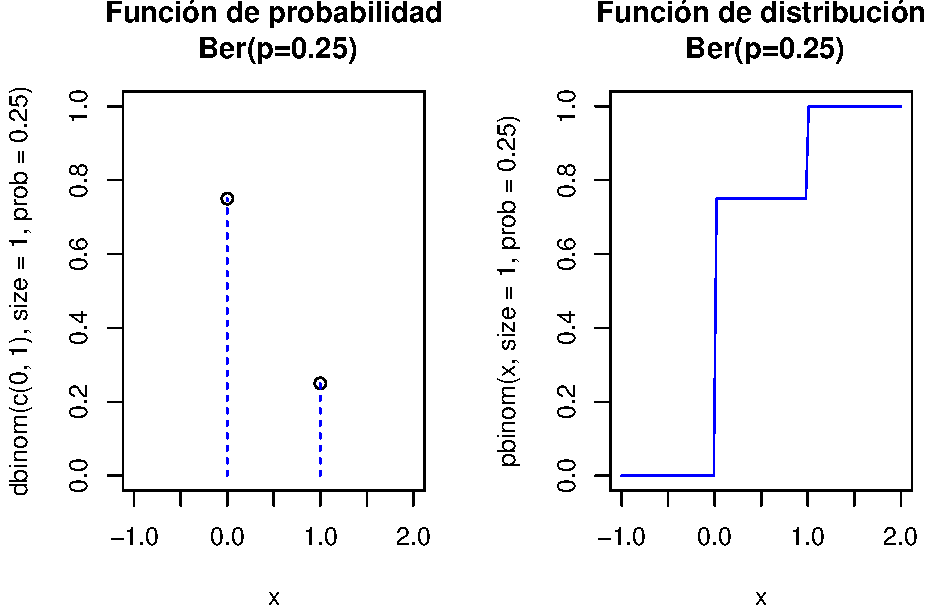
\includegraphics{distribuciones_notables_discretas_files/figure-latex/unnamed-chunk-4-1.pdf}

\hypertarget{distribuciuxf3n-binomial}{%
\subsection{Distribución binomial}\label{distribuciuxf3n-binomial}}

Si repetimos \(n\) veces de forma independiente un experimento Bernoulli
de parámetro \(p\). Se conoce a priori cuantas veces se tirará la
moneda.

El espacio muestral \(\Omega\) estará formado por cadenas \(E^{'} s\) y
\(F^{s}\) de longitud \(n\) consideremos la v.a.
\[X(EFF\ldots EEF) \; = \; \mbox{número de éxitos en la cadena}\]

\hypertarget{funciuxf3n-de-probabilidad-de-una-binomial}{%
\subsubsection{Función de probabilidad de una
binomial}\label{funciuxf3n-de-probabilidad-de-una-binomial}}

\[P_X(x)\left\{\begin{array}{rcl}
  {n \choose x}\cdot p^x \cdot (1-p)^{n-x}&si&x=0,1,\ldots,n\\
  0&si&\mbox{en otro caso}\\
\end{array}\right.\]

\hypertarget{funciuxf3n-de-distribuciuxf3n}{%
\subsubsection{Función de
distribución}\label{funciuxf3n-de-distribuciuxf3n}}

Su función de distribución no tiene una fórmula cerrada. Hay que
acumular la función de probabilidad:
\[F_X(x) = P(X\leq x) = \sum_{i=0}^x P_X(i)\]

\[P_X(x)\left\{\begin{array}{rcl}
  0&si&\\
  \sum_{i=1}^k {n \choose i} \cdot p^i \cdot (1-p)^{n-i}&si&k\leq x < k+1 \quad y \quad k=0,1,\ldots, n\\
  1&si&n\leq x\\
\end{array}\right.\]

\begin{Shaded}
\begin{Highlighting}[]
\CommentTok{\# Cuantas maneras distintas hay para elegir 5 jugadores en un conjunto de 6 jugadores. Todo el múndo diría 6!!!!. Efectivamente con R es}
\FunctionTok{choose}\NormalTok{(}\DecValTok{6}\NormalTok{,}\DecValTok{5}\NormalTok{)}
\end{Highlighting}
\end{Shaded}

\begin{verbatim}
## [1] 6
\end{verbatim}

\begin{Shaded}
\begin{Highlighting}[]
\CommentTok{\# con 10 jugadores el número de equipos de 5 distintos es bastante más grande}
\FunctionTok{choose}\NormalTok{(}\DecValTok{10}\NormalTok{,}\DecValTok{5}\NormalTok{)}
\end{Highlighting}
\end{Shaded}

\begin{verbatim}
## [1] 252
\end{verbatim}

\begin{Shaded}
\begin{Highlighting}[]
\CommentTok{\# Y por ejemplo con un equipo de fútbol profesional que tiene en plantilla 22 jugadores (quitamos el portero) se puede formar nada menos que:}
\FunctionTok{choose}\NormalTok{(}\DecValTok{22}\NormalTok{,}\DecValTok{10}\NormalTok{)}
\end{Highlighting}
\end{Shaded}

\begin{verbatim}
## [1] 646646
\end{verbatim}

Se denotará por \[X\equiv B(n,p)\]

Obviamente se tiene que una bernoulli es una binomial con \(n=1\)
\[B(1,p) \equiv Ber(p)\]

\hypertarget{esperanza-de-un-x-bnp}{%
\subsubsection{Esperanza de un X B(n,p)}\label{esperanza-de-un-x-bnp}}

Su esperanza es
\[E(X) = \sum_{k=0}^n k\cdot {n \choose k}\cdot p^k \cdot q^{n-k} = n\cdot p\]

La esperanza de \(X^2\) es
\[E(X^2) = \sum_{k=0}^n k^2\cdot {n\choose k}\cdot p^k \cdot q^{n-k} = n\cdot p\cdot q - (n\cdot p)^2\]

\hypertarget{varianza-de-una-x-bnp}{%
\subsubsection{Varianza de una X B(n,p)}\label{varianza-de-una-x-bnp}}

Su varianza es
\[Var(X) = E(X^2) - E^2(X) = n\cdot p\cdot q = n\cdot p \cdot (1-p)\]

Su desviación típica es
\[\sqrt{n\cdot p \cdot q} = \sqrt{n\cdot p \cdot (1-p)}\]

\hypertarget{la-distribuciuxf3n-binomila-en-python-y-r}{%
\subsection{La distribución Binomila en Python y
R}\label{la-distribuciuxf3n-binomila-en-python-y-r}}

\hypertarget{cauxe1culos-binomila-con-r}{%
\subsubsection{Caáculos binomila con
R}\label{cauxe1culos-binomila-con-r}}

Veamos los cálculos con funciones de R para una v.a. X con distribución
binomial B(n=10,p=0.25)

Si queremos calculo con R algún valor de la función de distribución como
por ejemplo \(F_X(0) = P(X\leq 0)\)

\begin{Shaded}
\begin{Highlighting}[]
\FunctionTok{pbinom}\NormalTok{(}\DecValTok{0}\NormalTok{,}\AttributeTok{size =} \DecValTok{10}\NormalTok{, }\AttributeTok{prob =} \FloatTok{0.25}\NormalTok{)}
\end{Highlighting}
\end{Shaded}

\begin{verbatim}
## [1] 0.05631351
\end{verbatim}

si queremos por ejemplo \(F_X(4) = P(X\leq 4)\)

\begin{Shaded}
\begin{Highlighting}[]
\FunctionTok{pbinom}\NormalTok{(}\DecValTok{4}\NormalTok{, }\AttributeTok{size =} \DecValTok{10}\NormalTok{, }\AttributeTok{prob =} \FloatTok{0.25}\NormalTok{)}
\end{Highlighting}
\end{Shaded}

\begin{verbatim}
## [1] 0.9218731
\end{verbatim}

Sin embargo, si queremos calcular algún valor de la función de
probabilidad como por ejemplo \(P(X=0)\)

\begin{Shaded}
\begin{Highlighting}[]
\FunctionTok{dbinom}\NormalTok{(}\DecValTok{0}\NormalTok{,}\AttributeTok{size=}\DecValTok{10}\NormalTok{, }\AttributeTok{prob =} \FloatTok{0.25}\NormalTok{)}
\end{Highlighting}
\end{Shaded}

\begin{verbatim}
## [1] 0.05631351
\end{verbatim}

o por ejemplo para \(P(X=4)\)

\begin{Shaded}
\begin{Highlighting}[]
\FunctionTok{dbinom}\NormalTok{(}\DecValTok{4}\NormalTok{, }\AttributeTok{size=}\DecValTok{10}\NormalTok{, }\AttributeTok{prob =} \FloatTok{0.25}\NormalTok{)}
\end{Highlighting}
\end{Shaded}

\begin{verbatim}
## [1] 0.145998
\end{verbatim}

\hypertarget{generaciuxf3n-de-muestras-aleatorias-con-r}{%
\subsubsection{Generación de muestras aleatorias con
R}\label{generaciuxf3n-de-muestras-aleatorias-con-r}}

Generaremos una muestra eleatoria de 100 valores de una población
B(20,0.5)

\begin{Shaded}
\begin{Highlighting}[]
\CommentTok{\# Repetir 100 veces el experimento lanzar una moneda 20 veces y contar el número de caras.}
\FunctionTok{set.seed}\NormalTok{(}\DecValTok{2021}\NormalTok{)}
\FunctionTok{rbinom}\NormalTok{(}\DecValTok{100}\NormalTok{, }\AttributeTok{size =} \DecValTok{20}\NormalTok{, }\AttributeTok{prob =} \FloatTok{0.5}\NormalTok{)}
\end{Highlighting}
\end{Shaded}

\begin{verbatim}
##   [1] 10 12 11  9 11 11 11  9 12 15  6 12 11 10 12  8 10 12 14 10  8 14  9  9 10
##  [26] 13 13 13 14 12  6 14 14 13 10  8 13  8 13 10  8 12 10 14  8 12 13  5  6 12
##  [51] 10 11  7 10  9  8 10  9 12 12  6 10  7  9 12  7  7 11  9  6  6 11  7 13  7
##  [76] 10 10  9 11 16 10  9 14 11  9  8 15 12 10  9  8 11 13 10  8 13 11 11 12 11
\end{verbatim}

\hypertarget{ejemplo-completo-de-distribuciuxf3n-binomial}{%
\subsection{Ejemplo completo de distribución
binomial}\label{ejemplo-completo-de-distribuciuxf3n-binomial}}

Tenemos una urna con 100 bolas de las cuales 40 son rojas y 60 blancas.
Extraemos al azar una bola, anotamos su color y la devolvemos (la
reponemos) a la urna Supongamos que repetimos este proceso \(n=10\)
reponiendo en cada ocación la bola extraida. Consideremos la v.a. \(X\)
= Número de bolas extraidas con repocisión en \(n=10\) repeticiones del
mismo experimento Bernoulli. Bajo estas condiciones tenemos que
repetimos \(n=10\) veces el mismo experimento Bernoulli con probabilidad
de éxito (sacar bola roja) es
\[P(Roja) = P(Exito)=p=\dfrac{40}{100}=0.4\]

Así que la variable \(X\) = número de bolas rojas extraídas de la urna
con reposición en \(n=10\) ocasiones sigue una ley binomial
\(B(n=10,p=0.4)\)

1.¿Cual es la probabilidad de que saquemos exactamente 4 rojas?

Respuesta.- Utilizando la función de probabilidad tenemos que
\[P_X(X=4) = {10 \choose 4} \cdot 0.4^4 \cdot (1-0.4)^10.4 = \dfrac{10!}{(10-4)!\cdot 4!}\cdot 0.4^4 \cdot 0.6^6 = 0.2508227\]

\begin{Shaded}
\begin{Highlighting}[]
\FunctionTok{dbinom}\NormalTok{(}\DecValTok{4}\NormalTok{, }\AttributeTok{size =} \DecValTok{10}\NormalTok{, }\AttributeTok{prob =} \FloatTok{0.4}\NormalTok{)}
\end{Highlighting}
\end{Shaded}

\begin{verbatim}
## [1] 0.2508227
\end{verbatim}

\begin{enumerate}
\def\labelenumi{\arabic{enumi}.}
\setcounter{enumi}{1}
\tightlist
\item
  ¿Cuál es la probabilidad de que saquemos al menos 4 rojas?
\end{enumerate}

Respuesta.- Al menos 4 rojas es
\(P(X\geq 4) = 1 - P(X<4) = 1 - P(X\leq 3)\) es decir,

\[\begin{array}{rcl}
    P(X\leq 3)&=&P(X=0) + P(X=1) + P(X=2) + P(X=3)\\\\
    &=&\displaystyle {10\choose 0}\cdot 0.4^0 \cdot (1-0.4)^{10-0} + {10\choose 1}\cdot 0.4^1 \cdot (1-0.4)^{10-1}\\\\ 
    &+& \displaystyle {10\choose 2}\cdot 0.4^2 \cdot (1-0.4)^{10-2} + {10\choose 3}\cdot 0.4^3 \cdot (1-0.4)^{10-3} \\\\
    &=&0.3822806\\\\
  \end{array}\]

\begin{Shaded}
\begin{Highlighting}[]
\FunctionTok{pbinom}\NormalTok{(}\DecValTok{3}\NormalTok{,}\DecValTok{10}\NormalTok{,}\FloatTok{0.4}\NormalTok{)}
\end{Highlighting}
\end{Shaded}

\begin{verbatim}
## [1] 0.3822806
\end{verbatim}

Así,
\(P(X\geq 4) = 1-P(X<4) = 1 - P(X\leq 3) = 1 - 0.3822806 = 0.6177194\)

\begin{Shaded}
\begin{Highlighting}[]
\DecValTok{1}\SpecialCharTok{{-}}\FunctionTok{pbinom}\NormalTok{(}\DecValTok{3}\NormalTok{,}\DecValTok{10}\NormalTok{,}\FloatTok{0.4}\NormalTok{)}
\end{Highlighting}
\end{Shaded}

\begin{verbatim}
## [1] 0.6177194
\end{verbatim}

Aunque en estos casos el parámetro lower.tail = FALSE es sin duda
nuestra mejor opción:

\begin{Shaded}
\begin{Highlighting}[]
\FunctionTok{pbinom}\NormalTok{(}\DecValTok{3}\NormalTok{,}\DecValTok{10}\NormalTok{,}\FloatTok{0.4}\NormalTok{,}\AttributeTok{lower.tail =} \ConstantTok{FALSE}\NormalTok{)}
\end{Highlighting}
\end{Shaded}

\begin{verbatim}
## [1] 0.6177194
\end{verbatim}

3.- ¿Cuál es la porbabilidad de que saquemos menos 3 rojas?

4.- ¿Cuál es el valor esperado del número de bolas rojas?

Respuesta.- Como \(X\) es una \(B(10,0.4)\) sabemos que
\[E(X) = n\cdot p = 10 \cdot 0.4 = 4\]

5.- ¿Cuál es la deviación típica del número de bolas rojas? La varianza
es \[Var(X) = n\cdot p \cdot (1-p) = 10\cdot 0.4 \cdot 0.6 = 2.4\] Y por
lo tanto \(\sqrt{Var(X)} = \sqrt{2.4} = 1.5491933\)

\hypertarget{distribuciuxf3n-geomuxe9trica}{%
\subsection{Distribución
geométrica}\label{distribuciuxf3n-geomuxe9trica}}

\begin{itemize}
  \item Repitamos un experimento Bernoulli de parámetro $p$, de forma independiente hasta obtener el primer éxito.
  \item Sea $X$ la v.a. que cuenta el número de fracasos antes del primer éxito. Por ejemplo que hayamos tenido $x$ fracasos será una cadena de $x$ fracasos culminada con un éxito. Más concretamente
  $$P(FFF, \ldots FE) = P(F)^x \cdot P(E) = (1-p)^x \cdot p = q^x \cdot p$$
  
\end{itemize}

\hypertarget{distribuciuxf3n-geomuxe9trica-1}{%
\subsubsection{Distribución
geométrica}\label{distribuciuxf3n-geomuxe9trica-1}}

Su función de probabilidad es
\[PX_(x) = P(X=x) = \left\{\begin{array}{rcl}
  (1-p)^x\cdot p&si&x=0,1,2,\ldots\\
  0&& \mbox{en otro caso}\\
\end{array}\right.\]

La denotaremos por \(Ge(p)\)

\hypertarget{funciuxf3n-de-distribuciuxf3n-1}{%
\subsubsection{Función de
distribución}\label{funciuxf3n-de-distribuciuxf3n-1}}

Calculemos \(P(X\leq 3)\).

Por la propiedad de la probabilidad del suceso complementario tenemos
que \[P(X\leq 3) = 1 -P(x>3) = 1-P(X\geq 4)\] Efectivamente, el evento
tenemos que \(X\leq 3\) es que hemos fracasado más de tres veces hasta
conseguir el primer éxito; es decir hemos gracasado 4 o más veces, por
lo tanto \[{X>3} = {X\geq4} = {FFFF}\]

Ahora al ser los intentos sucesos independientes, tenemos que:
\[\begin{array}{rcl}
  P(X>3)&=&P({FFFF}) = P(F)\cdot P(F)\cdot P(F)\cdot P(F)\\
  &=&(1-p)\cdot (1-p)\cdot (1-p)\cdot (1-p) = (1-p)^{3+1} \\
  &=&(1-p)^4\\
\end{array}\]

calculamos \[F_X(3) = P(X\leq 3) = 1-P(X>3) = 1-(1-p)^{3+1}\]

por lo que podemos generalizar a cualquier entero positivo
\(k=0,1,2,\ldots\)

\[F_X(x) = P(X\leq x) = \left\{\begin{array}{rcl}
  0&si&x<0\\\\
  1-(1-p)&si&k= 0 \leq x < 1\\\\
  1-(1-p)^2&si& k = 1\leq x < 2\\\\
  1-(1-p)^3&si& k = 2\leq x < 3\\\\
  1-(1-p)^{k+1}&si& k\leq x < k+1 \; para \; k=0,1,2,\ldots\\
\end{array}\right.\]

notemos que si \(k=0,1,2,\ldots\) el límite de la función de
distribución es
\[\lim_{k\to \infty} F_X(k) = \lim_{k\to \infty} 1 - (1-p)^{k+1} = 1\]

ya que \(0<1-p<1\)

\hypertarget{la-esperanza-y-la-varianza-de-una-distribuciuxf3n-geomuxe9trica.}{%
\subsection{La esperanza y la varianza de una distribución
geométrica.}\label{la-esperanza-y-la-varianza-de-una-distribuciuxf3n-geomuxe9trica.}}

\hypertarget{esperanza-de-una-v.a.-gep}{%
\subsubsection{Esperanza de una v.a.
Ge(p)}\label{esperanza-de-una-v.a.-gep}}

\[\begin{array}{rcl}
  E(X) &=& \sum\limits_{x=0}^\infty x \cdot P_X(x)\\
  &=& \sum\limits_{x=0}^\infty x\cdot (1-p)^x \cdot p\\\
  &=& p\cdot (1-p)\cdot \sum\limits_{x=1}^\infty x\cdot (1-p)^{x-1}\\
  &=& p\cdot (1-p)\cdot \dfrac{1}{\left[1-(1-p)\right]^2}\\
  &=&(1-p)\cdot \dfrac{1}{p^2}\\
  &=&\dfrac{1-p}{p}\\
\end{array}\]

\hypertarget{valor-ex2-de-una-v.a.-gep}{%
\subsubsection{Valor E(X\^{}2) de una v.a.
Ge(p)}\label{valor-ex2-de-una-v.a.-gep}}

\[\begin{array}{rcl}
  E(X^2) &=& \sum\limits_{x=0}^\infty x^2 \cdot P_X(x)\\\\
  &=& \sum\limits_{x=0}^\infty x^2 \cdot (1-p)^x \cdot p\\\\
  &=& \sum\limits_{x=1}^\infty \left[x\cdot (x-1)+x \right] (1-p)^{x} \cdot p\\\\
  &=&\sum\limits_{x=1}^\infty x\cdot (x-1)\cdot (1-p)^x\cdot p + \sum\limits_{x=1}^\infty x\cdot (1-p)^x \cdot p\\\\
  &=&(1-p)^2\cdot p \cdot \sum\limits_{x=2}^\infty x\cdot (x-1)\cdot (1-p)^{x-2}\\\\
  &+&(1-p)\cdot p\sum\limits_{x=1}^\infty x\cdot (1-p)^{x-1} \\\\
  &=&p\cdot (1-p)^2 \dfrac{2}{\left[1-(1-p)\right]^3} + (1-p)\cdot p \dfrac{1}{\left[1-(1-p)\right]^2}\\\\
  &=&p\cdot (1-p)^2 \dfrac{2}{p^3}+(1-p)\cdot p \dfrac{1}{p^2}\\\\
  &=&\dfrac{2\cdot(1-p)^2}{p^2}+\dfrac{1-p}{p}\\
\end{array}\]

\hypertarget{varianza-de-una-v.a.-gep}{%
\subsubsection{Varianza de una v.a.
Ge(p)}\label{varianza-de-una-v.a.-gep}}

\[\begin{array}{rcl}
  Var(X)&=&E(X^2) - E^2(X)\\\\
  &=&\dfrac{2\cdot(1-p)^2}{p^2}+\dfrac{1-p}{p}-\left(\dfrac{1-p}{p}\right)^2\\\\
  &=&\dfrac{2\cdot(1-p)^2+p\cdot (1-p)-(1-p)^2}{p^2}\\\\
  &=&\dfrac{(1-p)^2 + p\cdot (1-p)}{p^2}\\\\
  &=&\dfrac{1-2\cdot p p^2 + p - p^2}{p^2}\\\\
  &=&\dfrac{1-p}{p^2}\\\\
\end{array}\]

\hypertarget{propiedad-de-falta-de-memoria}{%
\subsection{Propiedad de falta de
memoria}\label{propiedad-de-falta-de-memoria}}

Sea \(X\) una v.a. discreta con dominio
\(D_X = \lbrace0,1,2, \ldots\rbrace\) con \(P(X=0) = p\) entonces \(X\)
sigue una ley \(Ge(p)\) si y sólo si
\[P(X> k + j \;|\; X\geq j) = P(X>k)\] para todo
\(k,j = 0,1,2,3,\ldots\)

Es decir, el número de veces que voy a fallar hasta el primer éxito no
está condicionado por las veces que estamos probando. Por ejemplo es lo
mismo lanzar 80 veces o lanzar 2 veces hasta el primer éxito.

Demostración.- Si es geométrica entonces el lado derecho de la igualdad
es \[P(X>k) = 1 - P(x\leq k) = 1 - (1-(1-p)^{k+1}) = (1-p)^{k+1}\]

Luego \[\begin{array}{rcl}
  P(X>k+j | X\geq j)&=&\dfrac{P(\lbrace X>k+j\rbrace)\cap \lbrace X\geq j\rbrace}{P(X\geq j)}\\\\
  &=&\dfrac{P(X>k+j)}{P(>\geq j)}\\\\
  &=&\dfrac{1-P(X\leq k+j)}{1-P(X\leq j-1)}\\\\
  &=&\dfrac{1-(1-(1-p)^{k+j+1})}{1-(1-(1-p)^{k-1+1})}\\\\
  &=&\dfrac{(1-p)^{k+j+1}}{(1-p)^j}\\\\
  &=&(1-p)^{k+1}\\\\
\end{array}\]

Para demostrar el recíproco tomemos \(j=1\) y \(k\geq 0\) entonces por
la propiedad de la pérdida de memoria \[P(X>k+1 | X\geq 1) = P(X>k)\]

Como sabemos \(P(X=0)=p\) tenemos
\(P(X\geq 1) = 1 - P(X<1) = 1-P(X=0) = 1-p\)

Luego combinando las igualdades tenemos que
\[P(X<k+1 | X\geq 1) = \dfrac{P(X>k+1, X\geq 1)}{P(X\geq 1)} = \dfrac{P(X>k+1)}{P(X\geq 1)} = P(X>k)\]

Así podemos poner que \[\begin{array}{rcl}
  P(X>k+1)&=&P(X\geq 1)\cdot P(X>k)\\\\
  &=&P(X<1)\cdot P(X>k)\\\\
  &=&(1-P(X=0))\cdot P(X>k)\\\\
  &=&(1-p)\cdot P(X>k)\\\\
\end{array}\]

En general tenemos que \[P(X>k+1) = (1-p)\cdot P(X>k)\]

del mismo modo para \(j=2\) \[P(X>k+2) = (1-p)\cdot P(X>k+1)\] Restando
la primera igualdad de la última obtenemos:
\[P(X>k+1) - P(X>k+2) = (1-p)\cdot P(X>k) - (1-p)\cdot P(X>k+1)\] de
donde operando en cada lado de la igualdad obtenemos la recurrencia
\[\left[1-P(X\leq k+1)  \right] - \left[1-P(X\leq k+2)\right] = (1-p)\cdot \left[P(X>k)-P(X>k+1)\right]\]

ahora operando \[\begin{array}{rcl}
  P(X\leq k+2)-P(X\leq k+1)&=&(1-p)\cdot \left[ 1-P(X\leq k)-(1-P(X\leq k+1))\right]\\\\
  P(X=k+2)&=&(1-p)\cdot \left[P(X\leq k+1)-P(X\leq k)\right]\\\\
  P(X=k+2)&=&(1-p)\cdot P(X=k+1)\\\\
\end{array}\]

De forma similar obtenemos \[P(X=k+1) = (1-p)\cdot P(X=k)\] Utilizando
la recurrencia anterior para calcular todas las probabilidades a partir
de la \(P(X=0)=p\); que vienen dadas por:

\[\begin{array}{rcl}
  P(X=0)&=&p\\
  P(X=1)&=&P(X=0+1) = (1-p)\cdot P(X=0) = (1-p)\cdot p\\
  P(X=2)&=&P(X=1+1) = (1-p)\cdot P(X=1)=(1-p)\cdot (1-p)\cdot p = (1-p)^2\cdot p\\
  P(X=k)&=&P(X=(k-1)+1) = (1-p)\cdot P(X=k+1) = (1-p)\cdot (1-p)^{k-1}\cdot p = (1-p)^k \cdot p\\
\end{array}\]

Lo que demuestra el recíproco, es decir que \(X\) es Geom(p).

\hypertarget{la-distribuciuxf3n-geomuxe9trica-con-r-y-python}{%
\subsection{La distribución geométrica con R y
Python}\label{la-distribuciuxf3n-geomuxe9trica-con-r-y-python}}

Veamos los cálculos básicos con R para la distribución geométrica
Ge(p=0.25). R implementa la geométrica que cuenta el número de fracasos.

\(P(X=0) = (1-0.25)^0 \cdot 0.25 = 0.25\)

\begin{Shaded}
\begin{Highlighting}[]
\FunctionTok{dgeom}\NormalTok{(}\DecValTok{0}\NormalTok{,}\AttributeTok{prob =} \FloatTok{0.25}\NormalTok{)}
\end{Highlighting}
\end{Shaded}

\begin{verbatim}
## [1] 0.25
\end{verbatim}

\(P(X\leq 0) = 1-(1-0.25)^{0+1} = 1 - 0.75 = 0.25\)

\begin{Shaded}
\begin{Highlighting}[]
\FunctionTok{pgeom}\NormalTok{(}\DecValTok{0}\NormalTok{,}\AttributeTok{prob =} \FloatTok{0.25}\NormalTok{)}
\end{Highlighting}
\end{Shaded}

\begin{verbatim}
## [1] 0.25
\end{verbatim}

\(P(X\leq 4) = 1-(1-0.25)^{4+1} = 1-0.75^5 = 0.7626953\)

\begin{Shaded}
\begin{Highlighting}[]
\FunctionTok{pgeom}\NormalTok{(}\DecValTok{4}\NormalTok{,}\AttributeTok{prob =} \FloatTok{0.25}\NormalTok{)}
\end{Highlighting}
\end{Shaded}

\begin{verbatim}
## [1] 0.7626953
\end{verbatim}

Una muestra de tamaño 25 de una Ge(0.25)

\begin{Shaded}
\begin{Highlighting}[]
\FunctionTok{rgeom}\NormalTok{(}\AttributeTok{n =} \DecValTok{25}\NormalTok{, }\AttributeTok{prob =} \FloatTok{0.25}\NormalTok{)}
\end{Highlighting}
\end{Shaded}

\begin{verbatim}
##  [1]  2 18  3  1  7  1  0 10  2  2  2  0  9  9  4  8  2  0  1  5  8  1  1  2  2
\end{verbatim}

\hypertarget{la-distribuciuxf3n-binomial-negativa}{%
\subsection{La distribución binomial
negativa}\label{la-distribuciuxf3n-binomial-negativa}}

\hypertarget{funciuxf3n-de-probabilidad}{%
\subsubsection{Función de
probabilidad}\label{funciuxf3n-de-probabilidad}}

\[P_X(x) = P(X=k) = \left\{\begin{array}{lcr}
  {k+n-1 \choose n-1}\cdot (1-p)^k \cdot p^n&si&k=0,1,\ldots\\\\
  0&&\mbox{en otro caso}\\
\end{array}\right.\]

\hypertarget{nuxfameros-binomiales-negativos}{%
\subsection{Números binomiales
negativos}\label{nuxfameros-binomiales-negativos}}

Dados dos enteros positivos \(n\) y \(k\) se define en número binomial
negativo como \[{-n\choose k} = \dfrac{(-n)(-n-1)\ldots (-n-k+1)}{k!}\]

se cumple que
\[(t+1)^{-n} = \sum\limits_{k=0}^{\infty} {-n \choose k} t^k\]

Con R es la misma función que para los números binomiales

\[{-6 \choose 4} = \dfrac{-6\cdot (-6-1)\cdot (-6-2) \cdot (-6-3) }{4!} = \dfrac{-6\cdot (-7)\cdot (-8)\cdot (-9)}{24} = \dfrac{3024}{24} = 126\]

\begin{Shaded}
\begin{Highlighting}[]
\FunctionTok{choose}\NormalTok{(}\SpecialCharTok{{-}}\DecValTok{6}\NormalTok{,}\DecValTok{4}\NormalTok{)}
\end{Highlighting}
\end{Shaded}

\begin{verbatim}
## [1] 126
\end{verbatim}

\hypertarget{esperanza-de-una-bnnp}{%
\subsubsection{Esperanza de una BN(n,p)}\label{esperanza-de-una-bnnp}}

Su esperanza es
\[E(X) = \sum\limits_{k=0}^\infty k \cdot {k+n-1 \choose n-1} \cdot (1-p)^k \cdot p^n = n\cdot \dfrac{1-p}{p}\]

La esperanza del cuadrado \(X^2\) es

\[E(X^2) = \sum\limits_{k=0}^\infty k^2 \cdot {k+n-1 \choose n-1} \cdot (1-p)^k \cdot p^n = n\cdot \dfrac{1-p}{p^2} + \left(n\cdot \dfrac{1-p}{p}\right)^2\]

\hypertarget{varianza-de-una-bnnp}{%
\subsubsection{Varianza de una BN(n,p)}\label{varianza-de-una-bnnp}}

Por último la varianza es
\[Var(X) = E(X^2)-E(X)^2 = n\cdot \dfrac{1-p}{p^2}+\left(n\cdot \dfrac{1-p}{p}\right)^2 - \left(n\cdot \dfrac{1-p}{p}\right)^2 = \dfrac{1-p}{p^2}\]

Y por tanto la desviación típica es
\[\sqrt{Var(X)} = \dfrac{\sqrt{n(1-p)}}{p}\]

\hypertarget{ejemplo-de-la-puerta-con-dos-llaves}{%
\subsection{Ejemplo de la puerta con dos
llaves}\label{ejemplo-de-la-puerta-con-dos-llaves}}

Tenemos un manojo de 10 llaves casi idénticas. De mnaera que cada vez
que probamos una llave olvidamos qué llave hemos usado. Sea \(X\) la
v.a. que nos da el número de intentos fallidos hasta abrir la puerta.

\hypertarget{section}{%
\paragraph{1.}\label{section}}

¿Cuál es la distribución de probabilidad de \(X\) la v.a. que nos da el
número de fallos hasta abrir la puerta? Respuesta.- Sabemos que la
probabilidad de éxito de cada intento es \(p=dfrac{1}{10} = 0.1\) Como
cada vez olvidamos qué llave hemos probado cada intento será
independiente del anterior. Así que la variable \(X\) que queremos
modelar cuenta el número de fallos de repeticiones sucesivas e
independientes de un experimento Ber(p=0.1) hasta conseguir 2 éxitos en
un experimento. Por lo tanto podemos asegurar que \(X\) sigue un
distribución BN(n=2,p=0.1)

\hypertarget{section-1}{%
\paragraph{2.}\label{section-1}}

¿Cuál es la función de probabilidad y de distribución de \(X\)?
Respuesta.- En general la función de probabilidad de un BN(n,p) es
\[P_X(x) = P(X=k) = \left\{ \begin{array}{ll}
  {k+n-1 \choose n-1}\cdot (1-p)^k \cdot p^n&si&k=0,1,\ldots\\\\
  0&&\mbox{en otro caso}\\
  \end{array}\right.\]

En particular la función de probabilidad de una BN(n=2,p=0.1) es
\[P_X(x) = P(X=k) = \left\{ \begin{array}{ll}
  {k+2-1 \choose 2-1}\cdot 0.9^k \cdot 0.1^2&si&k=0,1,\ldots\\\\
  0&&\mbox{en otro caso}\\
  \end{array}\right.\]

La función de distribución en general es
\[F_X(x) = P(X\leq x) = \left\{\begin{array}{lcl}
    0&si&\\
    \sum\limits_{i=1}^k {i+n-1 \choose n-1}\cdot \left(1-p\right)^{i+n-1}\cdot 0.1^n&si&x<0\\
    &si&k\leq x < k+1 \; y \; k=0,1,2,\ldots\\
    1&si&\mbox{en otro caso}\\
  \end{array}\right.\]

Para \(n=2\) y \(p=0.1\)

\[F_X(x) = P(X\leq x) = \left\{\begin{array}{lcl}
    0&si&\\
    \sum\limits_{i=1}^k {i+1 \choose 1}\cdot 0.9^{i+1}\cdot 0.1^2&si&x<0\\
    &si&k\leq x < k+1 \; y \; k=0,1,2,\ldots\\
    1&si&\mbox{en otro caso}\\
  \end{array}\right.\]

\hypertarget{section-2}{%
\paragraph{3.}\label{section-2}}

¿Cuál es la probabilidad de fallar exactamente 5 veces antes de abrir la
puerta? Respuesta.-
\[P(X=5) = {5+2-1\choose 1}\cdot 0.9^5 \cdot 0.1^2 = {6\choose 1}\cdot 0.9^5 \cdot 0.1^2 = 6\cdot 0.9^5 \cdot 0.1^2 = 0.0354294\]

\hypertarget{section-3}{%
\paragraph{5.}\label{section-3}}

¿Cuál es la probabilidad de fallar más de 4 ? Respuesta.-; Nos piden que
\[P(X>4) = 1 - P(X\leq 4)\] Calculemos primero \(P(X\leq 4):\)
\[\begin{array}{rcl}
    P(X\leq 4)&=&\sum\limits_{x=0}^4 P(X=x)\\\\
    &=&P(X=0) + P(X=1) + P(X=2) + P(X=3) + P(X=4)\\\\
    &=&{0+2-1\choose 1}\cdot 0.9^0 \cdot 0.1^2 + {1+2-1 \choose 1}\cdot 0.9^1 \cdot 0.1^2\\\\
    &+&{0+2-1\choose 1}\cdot 0.9^2 \cdot 0.1^2 + {1+2-1 \choose 1}\cdot 0.9^3 \cdot 0.1^2\\\\
    &+&{0+2-1\choose 1}\cdot 0.9^4 \cdot 0.1^2 \\\\
    &=&0.114265\\\\
  \end{array}\]

\hypertarget{section-4}{%
\paragraph{5.}\label{section-4}}

¿Cuál es el número esperado de fallos? ¿Y su desviación típica?
Respuesta.- Como \(X\) sigue una ley BN(n=2,p=0.1)
\[E(X) = n\cdot \dfrac{1-p}{p} = 2 \cdot \dfrac{1-0.1}{0.1} = 18\]

El número de fallos esperado es 18

\[Var(X) = n\cdot \dfrac{1-p}{p^2} = 2\cdot \cdot \dfrac{1-0.1}{0.1^2} = 180\]

Y su desviación típica será \[sv(X) = \sqrt{180}\]

\end{document}
